\section{Auswertung}

Wir betrachten zunächst das Resultat der Untergrundmessung, dieses ist in \abbref{plot:untergrund} zu sehen.

\begin{figure}[H]
    \centering
    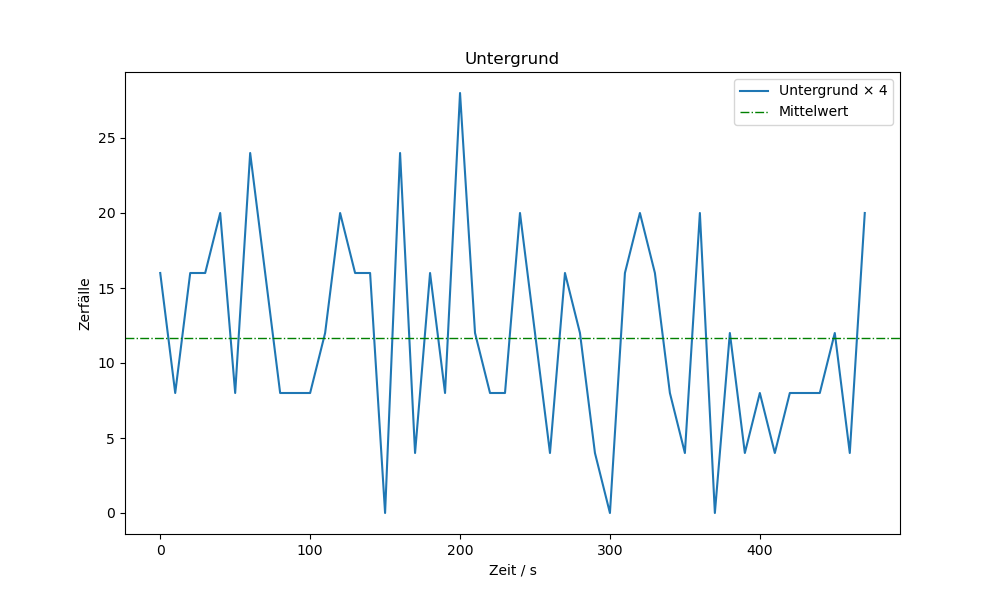
\includegraphics[width=.9\textwidth]{files/untergrund.png}
    \caption{Vervierfachter Untergrund mit Mittelwert}
    \label{plot:untergrund}
\end{figure}

Den Mittelwert des Untergrundes, im Plot in grün dargestellt, speichern wir uns ab für die Fits im weiteren Verlauf.

\subsection{Bestimmung der Halbwertszeit von aktiviertem Silber}

Zur Auswertung betrachten wir die Summe der vier Messgänge des Silberzerfalls. Da sich das aktivierte Silber aus zwei Isomeren mit unterschiedlichen Zerfallsverhalten zusammensetzt, fitten wir die Summer zweier Funktionen an die Daten. Die Fitfunktion für die Aktivität ist daher wie folgt definiert:
% A1*np.exp(-x*l1) + A2*np.exp(-x*l2) + y0
\begin{align}
A(t) = A_1 \e{-\lambda_1 t} + A_2 \e{-\lambda_2 t} + y_0 \label{eq:doulbe_exp_fit_func}
\end{align}

Hierbei sind $A_1$ und $A_2$ die anfänglichen Anzahlen verfügbarer radioaktiver Kerne, $\lambda_1$ und $\lambda_2$ die Zerfallskonstanten und $y_0$ der Offset, bestimmt durch den Mittelwert des Untergrundrauschens. Alle Variablen mit Index $1$ beziehen sich auf $^{110}$Ag, alle mit Index 2 auf $^{108}$Ag.


% Als Startparameter für den Fit verwenden wir die Werte aus Tabelle \ref{tab:fit_silver_startparams}.
% % 500,0.02,50,0.001
% \begin{table}[H]
%     \centering
%     \begin{tabular}{c|c}
%         Parameter & Startwert\\\hline
%         $A_1$ & $500$\\
%         $\lambda_1$ & $0.02$\\\hline
%         $A_2$ & $50$\\
%         $\lambda_2$ & $0.001$
%     \end{tabular}
%     \caption{Startparameter des Fits an die Aktivität des aktivierten Silbers}
%     \label{tab:fit_silver_startparams}
% \end{table}

\abbref{plot:fit_silber} zeigt die Daten des Silberzerfalls, gemeinsam mit der angepassten Funktion aus Gleichung \ref{eq:doulbe_exp_fit_func}. Die optimierten Parameter sind \tabref{tab:fit_silver_fitted} zu entnehmen.

\begin{figure}[H]
    \centering
    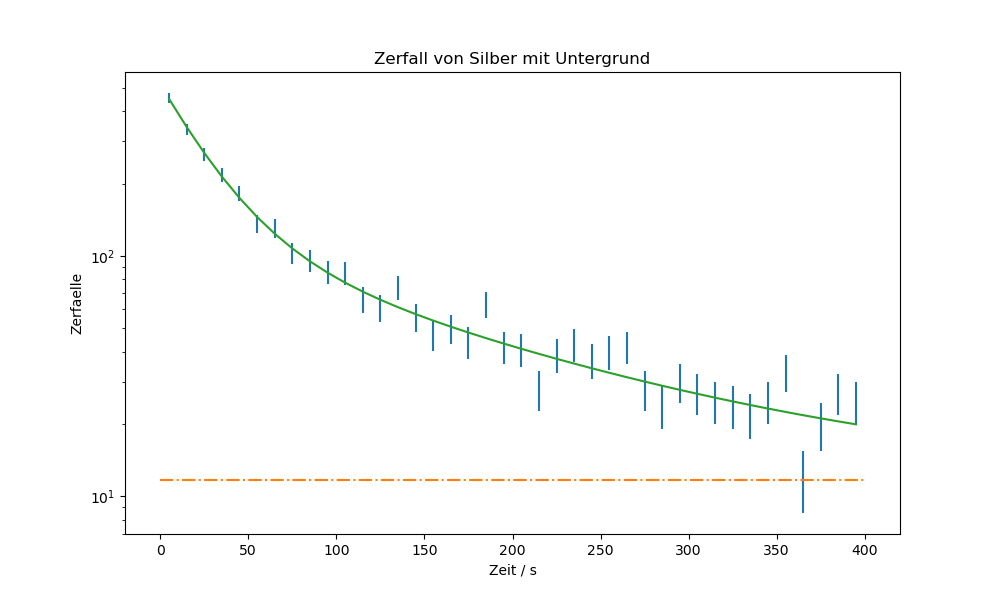
\includegraphics[width=.9\textwidth]{files/silber.png}
    \caption{Fit der Aktivität von aktiviertem Silber}
    \label{plot:fit_silber}
\end{figure}

\begin{table}[H]
    \centering
    \begin{tabular}{c|c}
        Parameter & Optimierter Wert\\\hline
        $A_1$ & $394 \pm 26$\\
        $\lambda_1$ & $(0.036 \pm 0.005) \si{\per\second}$\\\hline
        $A_2$ & $114 \pm 20$\\
        $\lambda_2$ & $(0.0066 \pm 0.0008) \si{\per\second}$
    \end{tabular}
    \caption{Optimierte Parameter für die Aktivität des aktivierten Silbers}
    \label{tab:fit_silver_fitted}
\end{table}

Zur Beurteilung der Güte des Fits berechnen wir die üblichen Werte $\chisq$, $\chisqrd$, sowie die Fitwahrscheinlichkeit $\mathbb{P}_{\mathrm{Fit}}$.
\begin{align}
    \chisq = 37.56, \qquad \chisqrd = 1.04, \qquad \mathbb{P}_{\mathrm{Fit}} = 40.0\%
\end{align}
Diese werden im abschließenden Teil der Ausarbeitung beurteilt werden.

Wie in Gleichung \ref{eq:doulbe_exp_fit_func} zu erkennen, geht der Mittelwert des Untergrunds als die Variable $y_0$ zwar in diesen Fit mit ein, allerdings nicht der Fehler des Untergrunds. Um auch diesen Fehler mit Berücksichtigen zu können, führen wir den eben dargestellten Fit noch zwei weitere Male durch. Einmal mit $y_0$ als Summe vom Mittelwert des Untergrundes und dessen Fehler und einmal als Differenz der Werte. Daraus erhalten wir für die Zerfallskonstanten weitere optimierte Werte $\lambda_1^+, \lambda_2^+$ für den addierten Fehler und $\lambda_1^-, \lambda_2^-$ für den subtrahierten Fehler. 

Nun Berechnen wir die Abstände zwischen diesen neuen Werten und den zuvor optimierten $\lambda_1, \lambda_2$ in der Form
\begin{align}
    \Delta^+_{bkg}(\lambda_i) &= |\lambda_i - \lambda_i^+|,\\
    \Delta^-_{bkg}(\lambda_i) &= |\lambda_i - \lambda_i^-|
\end{align}
und erhalten den gesamten Fehler durch den Untergrund als den Mittelwert der Abstände
\begin{align}
    \Delta_{bkg}(\lambda_i) = \frac{\Delta^+_{bkg}(\lambda_i) + \Delta^-_{bkg}(\lambda_i)}{2}.
\end{align}

Diese Fehlerwerte summieren wir nun quadratisch mit den unsprünglich durch den Fit für $\lambda_i$ bestimmten Fehlern nach
\begin{align}
    \Delta \lambda_i &= \sqrt{\Delta_{fit}(\lambda_i)^2 + \Delta_{bkg}(\lambda_i)^2}
\end{align}
auf, um den gesamten Fehler der Zerfallskonstanten zu erhalten. Somit können wir nun die Zerfallskonstanten wie folgt angeben:
\begin{align}
    \lambda_1 &= (0.036 \pm 0.005)\, \si{\per\second},\\[1em]
    \lambda_2 &= (0.0066 \pm 0.0009)\, \si{\per\second}.
\end{align}

Aus diesen Werten berechnen wir die Halbwertszeiten nach
\begin{align}
    T_{\flatfrac{1}{2}, i} = \frac{\ln{2}}{\lambda_i} \pm \frac{\ln{2}}{\lambda_i^2} \Delta \lambda_i
\end{align}
und erhalten
\begin{align}
    T_{\flatfrac{1}{2}, 1} &= (19.3 \pm 1.7)\, \si{\second},\\[1em]
    \intertext{als Halbwertszeit von $^{110}$Ag und}
    T_{\flatfrac{1}{2}, 2} &= (105 \pm 9)\, \si{\second}.
\end{align}
als Halbwertszeit von $^{108}$Ag.

Im abschließenden Diskussionsteil werden diese Werte mit den Literaturwerten verglichen werden. Zunächst fahren wir jedoch damit fort, die Halbwertszeit des Indiumisotops zu berechnen.

\subsection{Bestimmung der Halbwertszeit von aktiviertem Indium}

Für den vorherigen Versuchsteil nahmen wir die Anzahl an Zerfällen in Intervallen (Torzeit) von zehn Sekunden auf. Entsprechend führten wir auch die Untergrundmessung über zehn Sekunden durch. Für die Messungen am aktivierten Indium wurde die Torzeit auf 120 Sekunden erhöht. Entsprechend multiplizieren wir den Mittelwert und den Fehler des Untergrunds mit 12, um entsprechende Werte für das größere Intervall zu erhalten.

Ab diesem Punkt gehen wir größtenteils analog zur Auswertung des Silberzerfalls vor. Als Modell für die Aktivität verwenden wir eine einfach Exponentialfunktion der Form
\begin{align}
    A(t) = A_0 \e{-\lambda t}.
\end{align}

Das Resultat des Fits ist in \abbref{plot:fit_indium} zu sehen, die optimierten Parameter sind erneut in der \tabref{tab:fit_indium_fitted} darunter.

\begin{figure}[H]
    \centering
    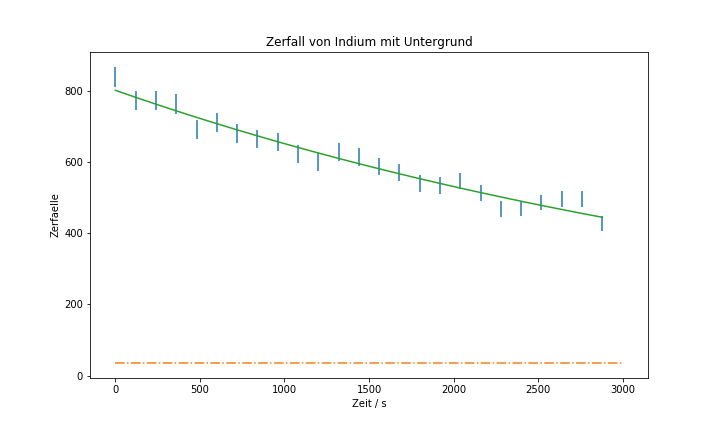
\includegraphics[width=.9\textwidth]{files/indium.png}
    \caption{Fit der Aktivität von aktiviertem Indium}
    \label{plot:fit_indium}
\end{figure}

\begin{table}[H]
    \centering
    \begin{tabular}{c|c}
        Parameter & Optimierter Wert\\\hline
        $A$ & $766 \pm 11$\\
        $\lambda$ & $(0.217 \pm 0.009) \cdot 10^{-3} \si{\per\second}$
    \end{tabular}
    \caption{Optimierte Parameter für die Aktivität des aktivierten Indiums}
    \label{tab:fit_indium_fitted}
\end{table}

Zur späteren Beurteilung der Güte des Fits in der Diskussion werden wir die Werte
\begin{align}
    \chisq = 17.7, \qquad \chisqrd = 0.84, \qquad \mathbb{P}_{\mathrm{Fit}} = 67.0\%
\end{align}
betrachten.

Auch für diesen Fit müssen wir wieder die Auswirkungen des Fehlers des Untergrundes auf den Fehler der Zerfallskonstanten separat berechnen. Hierzu gehen wir analog zum vorherigen Versuchsteil vor und erhalten damit einen Wert für die Zerfallskonstante von
\begin{align}
    \lambda = (0.217 \pm 0.009) \cdot 10^{-3} \si{\per\second}.
\end{align}

Der Fehler durch den Untergrund ist hier mit $\Delta_{bkg}(\lambda) = 1.2 \cdot 10^{-6}$ so gering, dass er nur außerhalb der signifikanten Stellen des Fehlers eine Auswirkung hat und somit, hier nicht ersichtlich ist.

Mit der soeben bestimmten Zerfallskonstante können wir nun abschließend die Halbwertszeit von Indium-116 zu
\begin{align}
    T_{\flatfrac{1}{2}} = 53.1 \pm 2.2\si{\minute}
\end{align}
bestimmen.